\section{Pregunta N$^{\circ}$3\qquad Carlos Alonso Aznarán Laos}

\begin{frame}
  \frametitle{Método explícito de Runge-Kutta}
  La derivación sistemática de los métodos de un paso de orden
  superior se remonta a Runge y Kutta, quienes desarrollaron métodos
  especiales de tercer y cuarto orden hace más de $122$ años.

  \

  \begin{definition}[Runge-Kutta explícito de $m$ etapas]
    Un método se denomina \alert{Runge-Kutta explícito de $m$ etapas}
    sii la función del método $f_{h}$ es una combinación lineal de
    valores de la función $f\left(x,y\right)$ en diferentes puntos
    $\left(x,y\right)$ es
    \begin{math}
      f_{h}\left(x,y\right)=
      \gamma_{1}k_{1}\left(x,y\right)+
      \gamma_{2}k_{2}\left(x,y\right)+
      \cdots+
      \gamma_{m}k_{m}\left(x,y\right)
    \end{math}
    con

    \

    \begin{columns}
      \begin{column}{0.48\textwidth}
        \begin{align*}
          k_{1}\left(x,y\right) & =
          f\left(
          x,y
          \right)                                 \\
          k_{2}\left(x,y\right) & =
          f\left(
          x+\alpha_{2}h,
          y+h\beta_{21}k_{1}\left(x,y\right)
          \right).                                \\
          k_{3}\left(x,y\right) & =
          f\left(
          x+\alpha_{3}h,
          y+h\left[\beta_{31}k_{1}\left(x,y\right)+\beta_{32}k_{2}\left(x,y\right)\right]
          \right)                                 \\
                                & \vdotswithin{=} \\
          k_{m}\left(x,y\right) & =
          f\left(x+\alpha_{m}h,y+h\sum\limits_{j=1}^{m-1}\beta_{mj}k_{j}\left(x,y\right)\right),
        \end{align*}
      \end{column}
      \begin{column}{0.48\textwidth}
        \begin{equation*}
          \begin{array}
            {c|ccccc}
            0                                                                    \\
            \alpha_{2} & \beta_{21}                                              \\
            \alpha_{3} & \beta_{31} & \beta_{32}                                 \\
            \vdots     & \vdots     &            & \ddots                        \\
            \alpha_{m} & \beta_{m1} & \beta_{m2} &        & \beta_{mm-1}         \\
            \hline
                       & h_{1}      & h_{2}      & \cdots & h_{m-1}      & h_{m}
          \end{array}
        \end{equation*}
        Este método será \alert{consistente} sii
        \begin{math}
          \sum\limits_{j=1}^{m}
          h_{j}=1
        \end{math}.
      \end{column}
    \end{columns}
    donde $x=x_{j}$, $y=u_{j}$ y $h=h_{j}$ para el paso $j$.

    \

    Por lo tanto, el método se determina fijando
    $2m-1+\dfrac{m\left(m-1\right)}{2}$ parámetros
    \begin{equation*}
      \left\{
      \gamma_{1},\dotsc,\gamma_{m},
      \alpha_{2},\alpha_{3},\dotsc,\alpha_{m},
      \beta_{21},\beta_{31},\beta_{41}\dotsc,\beta_{mm-1}
      \right\}\subset
      \mathbb{R}.
    \end{equation*}
  \end{definition}
\end{frame}

\begin{frame}
  \frametitle{Método de Heun de orden 2}
  El método clásico de Heun es
  \begin{align*}
    \overline{u_{j+1}} & =
    u_{j}+
    hf\left(x_{j},u_{j}\right). \\
    u_{j+1}            & =
    u_{j}+
    \frac{h}{2}
    \left[
      f\left(x_{j},u_{j}\right)+
      f\left(t_{j+1},\overline{u_{j+1}}\right)
      \right],
  \end{align*}

  donde $h$ es el tamaño de paso y $x_{j+1}=x_{j}+h$.
  Y tiene la siguiente representación en la tabla de Butcher:
  % Tenemos para $m=4$, $2\times 4-1+\dfrac{4\left(4-1\right)}{2}=13$
  % parámetros, $11$ condiciones.
  \begin{equation*}
    \renewcommand\arraystretch{1.3}
    \begin{array}
      {c|cc}
      0 & 0           & 0           \\
      1 & 1           & 0           \\
      \hline
        & \frac{1}{2} & \frac{1}{2}
    \end{array}
  \end{equation*}
\end{frame}

\begin{frame}[fragile]
    \begin{enumerate}\setcounter{enumi}{2}
        \item

              Resuelva el problema de valor inicial

              \begin{equation*}
                  \begin{cases}
                      \diff{y}{x}=\frac{3x-2y\left(x\right)}{x},
                       & x\in\left[1,2\right]. \\
                      y\left(1\right)=0.
                       &
                  \end{cases}
              \end{equation*}
              usando el método de Heun con tamaño de paso $h=0.1$.
    \end{enumerate}

    \begin{solution}
        \begin{columns}
            \begin{column}{0.38\textwidth}
                \inputminted[fontsize=\tiny,firstline=3,lastline=4]{python}{p3.py}
                \inputminted[fontsize=\tiny,firstline=10,lastline=11]{python}{p3.py}
                \inputminted[fontsize=\tiny,firstline=14,lastline=15]{python}{p3.py}
                \inputminted[fontsize=\tiny,firstline=18,lastline=21]{python}{p3.py}
                \inputminted[fontsize=\tiny,firstline=23,lastline=25]{python}{p3.py}
            \end{column}
            \begin{column}{0.58\textwidth}
                \inputminted[fontsize=\tiny,firstline=28,lastline=31]{python}{p3.py}
            \end{column}
        \end{columns}
    \end{solution}
\end{frame}

\begin{frame}
    \begin{solution}
        \begin{figure}[ht!]
            \centering
            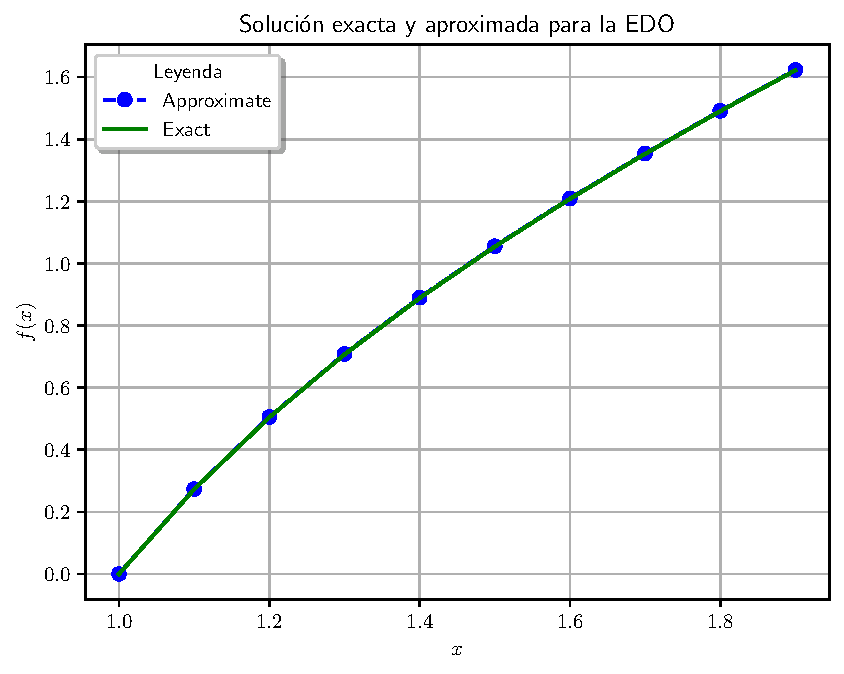
\includegraphics[width=0.65\paperwidth]{p3}
        \end{figure}
    \end{solution}
\end{frame}